\documentclass[conference]{IEEEtran}
\usepackage[T1]{fontenc}
\usepackage[utf8]{inputenc}
\usepackage{cite}
\usepackage{graphicx}
\usepackage{booktabs}
\usepackage{array}
\usepackage{amsmath,amssymb}
\usepackage{url}
\usepackage{float}

\title{Is the Spline-Angle Claim Actually Reproduced?\\A Regime-Sensitive Reassessment of WVF/LF Orientation Estimation}

\author{\IEEEauthorblockN{Reproduction Study}
\IEEEauthorblockA{Edge-Detection Filter Critique Project}}

\begin{document}
\maketitle

\begin{abstract}
The WVF/LF papers claim that replacing the usual arctangent-based gradient direction estimate with a cubic-spline angle estimate improves edge orientation accuracy, especially in noisy aquatic imagery. This paper re-examines that claim using the local synthetic angle sweep artifact \texttt{angle\_sweep\_paperlike\_v2}, which spans five support sizes, three orientation discretizations, and four signal-to-noise levels. The resulting 60-row sweep does not support a blanket statement of uniform superiority. Instead, the spline estimate is regime dependent: small support (\(N_p=15\)) is often worse than the Sobel/atan baseline, moderate support (\(N_p=50\) and \(N_p=100\)) is the most promising region, and very large support (\(N_p=250\)) can recover gains only at substantial runtime cost. The best observed case improves mean angular error by \(21.99^{\circ}\), while the worst case regresses by \(8.69^{\circ}\). Averaged over all four noise settings, \(N_p=50\) yields the strongest improvement/performance balance, whereas \(N_p=250\) is computationally expensive enough that its modest average gains are difficult to justify. The evidence supports a narrower conclusion: spline-based angle estimation is sometimes helpful, but it is not uniformly superior.
\end{abstract}

\begin{IEEEkeywords}
edge detection, gradient orientation, cubic spline interpolation, WVF, LF, reproduction study, signal-to-noise ratio
\end{IEEEkeywords}

\section{Introduction}
Accurate edge orientation is a foundational problem in classical vision. In the Canny pipeline, gradient direction is used to suppress non-maximal responses and to localize edges consistently \cite{canny1986}. Related subpixel edge localization methods also depend on the idea that better local geometry improves downstream edge quality \cite{trujillo2013}. The WVF/LF line of work makes a stronger claim: by replacing the conventional arctangent angle estimate with a cubic-spline interpolation over wide-view gradient samples, the method should estimate orientation more accurately, particularly when local measurements are noisy or low contrast \cite{bagan2023thesis,bagan2025wvf,bagan2025msmd}.

That claim matters because it is easy to overstate. A better angle estimator can help an edge detector only if the support size, orientation sampling, and noise regime are all favorable. A method that is better in one regime and worse in another is not a uniformly superior replacement. This paper tests exactly that boundary.

Our contribution is deliberately narrow:
\begin{itemize}
    \item We isolate the angle-estimation claim from the rest of the edge-detection stack.
    \item We summarize the local angle sweep across \(N_p \in \{15,50,100,150,250\}\), three orientation counts, and four SNR levels.
    \item We identify the best and worst sweep rows, the mean improvement by support size, and the runtime cost of the high-support cases.
    \item We state the result plainly: spline-based angle estimation is sometimes helpful, but it is not uniformly superior.
\end{itemize}

\section{Source Claim and Reproduction Protocol}
The thesis introduces WVF and LF as wide-support gradient operators intended to improve derivative quality in noisy imagery \cite{bagan2023thesis}. The 2025 WVF/LF conference paper frames the spline-based angle estimate as a means to improve gradient orientation computation, and the later 2025 paper extends the idea into a multi-scale, multi-domain system with Gaussian-mixture fusion \cite{bagan2025wvf,bagan2025msmd}. The common claim across these works is that spline-based orientation is more accurate than the standard Sobel/\(\arctan\) path when the local support is chosen appropriately.

The sweep used here is a controlled synthetic test rather than a full end-to-end edge detector benchmark. Each row compares the mean angular error of the Sobel/atan baseline against the spline-angle estimate for a fixed \((N_p, N_o, \mathrm{SNR})\) setting, where \(N_o\) is the number of sampled orientations. The local artifact contains 60 rows in total, covering:
\begin{itemize}
    \item support sizes \(N_p \in \{15,50,100,150,250\}\),
    \item orientation counts \(N_o \in \{18,36,72\}\),
    \item SNR levels \(\{2.0,1.0,0.75,0.5\}\).
\end{itemize}

This design is intentionally stricter than a narrative claim and less ambitious than a full reproduction of the final paper stack. It tests the local angle estimator directly, which is the only fair way to answer the question: does the spline angle itself improve orientation estimation, and if so, when?

\begin{figure*}[t]
    \centering
    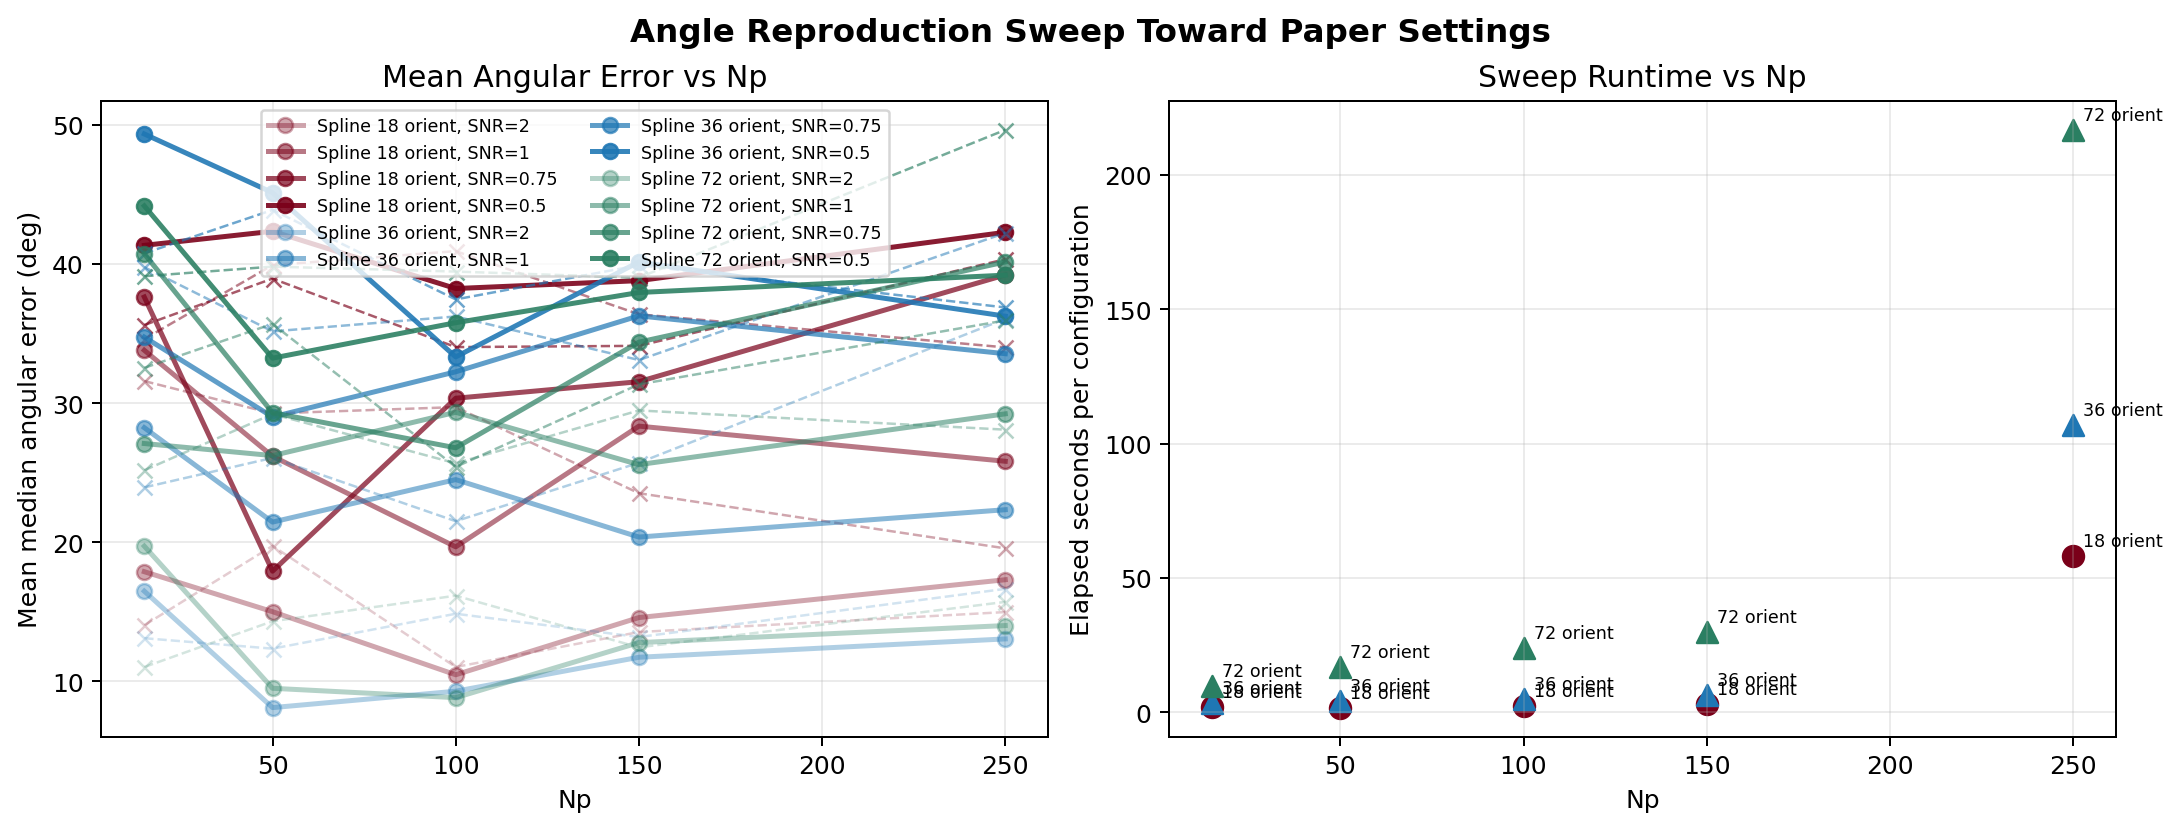
\includegraphics[width=\textwidth]{../../../benchmarks/angle_sweep_results/angle_sweep_paperlike_v2.png}
    \caption{Local angle sweep summary. Positive values indicate that the spline estimate reduced angular error relative to the Sobel/atan baseline; negative values indicate regression. The figure makes the core result visible immediately: the spline path helps in some regimes and hurts in others.}
    \label{fig:sweep}
\end{figure*}

\section{Results}
\subsection{The sweep is regime-sensitive, not monotone}
Figure~\ref{fig:sweep} is the central result. There is no global monotonic improvement with support size or with orientation density. The sweep contains clear positive regions, clear negative regions, and several boundary cases in which the spline estimate is nearly neutral.

The mean improvement by support size is summarized in Table~\ref{tab:support}. Two things stand out. First, \(N_p=15\) is counterproductive on average: the spline estimate loses \(4.16^{\circ}\) relative to Sobel. Second, \(N_p=50\) is the best average trade-off in this sweep, improving by \(5.08^{\circ}\) at a moderate runtime cost. \(N_p=100\) remains positive but weaker. \(N_p=150\) is effectively neutral, and \(N_p=250\) is only mildly positive on average while becoming much slower.

\begin{table}[t]
    \centering
    \caption{Mean angular improvement by support size. Positive values favor the spline estimate. Runtime is the average per row in the sweep.}
    \label{tab:support}
    \begin{tabular}{@{}rcc@{}}
        \toprule
        \(N_p\) & Mean improvement (\(^\circ\)) & Mean runtime (s) \\
        \midrule
        15  & -4.16 & 4.95 \\
        50  & +5.08 & 7.55 \\
        100 & +2.80 & 10.47 \\
        150 & -0.06 & 13.14 \\
        250 & +1.47 & 127.27 \\
        \bottomrule
    \end{tabular}
\end{table}

The noise dependence is also nontrivial. The mean improvement is positive at SNR \(2.0\), \(1.0\), and \(0.75\), but it turns negative at SNR \(0.5\). The largest average gain occurs at SNR \(0.75\), not at the noisiest setting. That is an important nuance: the spline estimate is not simply ``more useful when noise is higher.'' It is useful in some mid-noise regimes and not automatically better as the signal degrades.

\subsection{Best and worst rows}
Table~\ref{tab:extrema} shows the most informative extrema. The best overall row is \(N_p=50\), \(N_o=18\), SNR \(0.75\), with a \(21.99^{\circ}\) reduction in mean angular error at \(1.70\) seconds. The worst row is \(N_p=15\), \(N_o=72\), SNR \(2.0\), which regresses by \(8.69^{\circ}\) and still takes almost \(9.77\) seconds.

Two additional facts strengthen the case against a universal claim. First, only two \((N_p,N_o)\) settings remain positive across all four SNR values: \((50,72)\) and \((250,36)\). Second, the second of those is expensive enough to blunt its practical value, averaging \(106.86\) seconds per row. This is the right reading of the evidence: there are settings where the spline angle is consistently beneficial, but they are not free and they are not universal.

\begin{table}[t]
    \centering
    \caption{Representative extrema and regime anchors from the angle sweep.}
    \label{tab:extrema}
    \small
    \begin{tabular}{@{}p{1.45in}cc@{}}
        \toprule
        Case & \(\Delta\) (\(^\circ\)) & Time (s) \\
        \midrule
        Best overall: \(N_p=50\), \(N_o=18\), SNR \(0.75\) & +21.99 & 1.70 \\
        Worst overall: \(N_p=15\), \(N_o=72\), SNR \(2.0\) & -8.69 & 9.77 \\
        Best at SNR \(2.0\): \(N_p=100\), \(N_o=72\) & +7.33 & 24.05 \\
        Best at SNR \(0.5\): \(N_p=250\), \(N_o=72\) & +10.44 & 216.78 \\
        \bottomrule
    \end{tabular}
\end{table}

\begin{figure}[t]
    \centering
    \includegraphics[width=\linewidth]{../../../results/angle_error_comparison.png}
    \caption{Representative angular-error comparison from the local angle study. The pattern is consistent with the sweep summary: the spline estimate can improve some cases substantially, but the improvement is not uniform across support sizes and noise levels.}
    \label{fig:errorcmp}
\end{figure}

\begin{figure}[t]
    \centering
    \includegraphics[width=\linewidth]{../../../results/angle_test_images.png}
    \caption{Synthetic test images used in the angle study. These examples are useful because they show the experimental regime directly: the reproduction tests the orientation estimator on controlled line targets rather than on a full end-to-end edge map.}
    \label{fig:testimages}
\end{figure}

\section{Runtime Cost}
The runtime story is as important as the accuracy story. The local sweep shows a steep growth in cost as \(N_p\) increases. Mean runtime rises from \(4.95\) seconds at \(N_p=15\) to \(127.27\) seconds at \(N_p=250\), a factor of more than \(25\times\). The slowest row in the sweep is \(N_p=250\), \(N_o=72\), SNR \(2.0\), which takes \(216.78\) seconds while improving the angle error by only \(1.70^{\circ}\).

This is the central practical trade-off: the largest-support configurations can recover some angle accuracy, but the cost grows much faster than the gains. The spline claim therefore has to be framed as a quality-speed trade-off, not as a free upgrade. If the application needs real-time throughput or if many images must be processed, the support regime matters as much as the estimator choice.

\section{Discussion}
The result is best stated carefully.

First, the spline angle estimator is \emph{not} uniformly superior. That is the strongest conclusion the sweep allows. There are rows where it improves angle error dramatically, and rows where it makes things worse. Any blanket claim to the contrary would be overstated.

Second, the estimator is \emph{sometimes helpful} in a meaningful sense. The best average support regime is \(N_p=50\), and several mid-support rows are positive across all SNR values. In particular, \((50,72)\) and \((250,36)\) are consistently positive across the four SNRs tested. So the spline is not a gimmick; it does improve orientation estimation in some settings.

Third, the improvement is conditional on scale matching. This is consistent with classical edge-detection intuition. Canny-style pipelines already depend on a good local orientation estimate \cite{canny1986}, and subpixel edge work shows that edge quality is sensitive to how local geometry is estimated \cite{trujillo2013}. The sweep here extends that lesson: if the support is too small, the spline underfits the structure; if the support is too large, the method becomes expensive and its average benefit diminishes.

Finally, this reproduction is intentionally narrow. It does not claim to re-create the full WVF/LF benchmark suite, BIPED results, or the later multi-domain GMM pipeline. It tests the one claim that can be isolated cleanly from the rest: does the spline angle estimate itself improve orientation accuracy? The answer is yes, sometimes, but not universally and not cheaply.

\section{Conclusion}
The local angle sweep does not justify a claim of uniform spline superiority. It does justify a narrower claim: spline-based angle estimation can improve gradient-orientation accuracy, especially in selected mid-support regimes, but it is highly sensitive to \(N_p\), orientation discretization, and noise level. The best average support size in this reproduction is \(N_p=50\); \(N_p=15\) is often worse than Sobel; \(N_p=150\) is effectively neutral; and \(N_p=250\) is too expensive to defend on accuracy alone.

If the source-paper statement is rewritten as ``spline angle estimation is sometimes helpful when the support is well matched to the local edge geometry,'' the evidence supports it. If the statement is rewritten as ``spline angle estimation is uniformly superior,'' the evidence does not.

\begin{thebibliography}{99}

\bibitem{canny1986}
J.~Canny, ``A computational approach to edge detection,'' \emph{IEEE Transactions on Pattern Analysis and Machine Intelligence}, vol.~PAMI-8, no.~6, pp.~679--698, Nov. 1986.

\bibitem{trujillo2013}
A.~D. Trujillo-Pino, K.~Krissian, M.~Alem\'an-Flores, and D.~Santana-Cedr\'es, ``Accurate subpixel edge location based on partial area effect,'' \emph{Image and Vision Computing}, vol.~31, no.~1, pp.~72--90, 2013.

\bibitem{bagan2023thesis}
L.~Bagan, \emph{Wide View and Line Filter for Enhanced Image Gradient Computation and Edge Determination}, M.S. thesis, University of South Carolina, 2023.

\bibitem{bagan2025wvf}
L.~Bagan, ``Wide View and Line Filter for Enhanced Gradient Computation in Aquatic Environment,'' in \emph{Proc. IEEE OCEANS 2025 Great Lakes}, 2025.

\bibitem{bagan2025msmd}
L.~Bagan, ``Multi-Scale and Multi-Domain Edge Determination with Accurate Gradient Orientation Computation in Aquatic Environment,'' in \emph{Proc. IEEE OCEANS 2025 Great Lakes}, 2025.

\end{thebibliography}

\end{document}
